% Бүлэг 1

\chapter{Системийн танилцуулга} % Бүлгийн нэр
\label{Chapter1} % Энэ бүлэг рүү ишлэл хийх бол \ref{Chapter1} командыг ашигла 

%-------------------------------------------------------------------------------

% Агуулгад ашигласан хэвшүүлэлтийн зарим командын тодорхойлолт
\newcommand{\keyword}[1]{\textbf{#1}}
\newcommand{\tabhead}[1]{\textbf{#1}}
\newcommand{\code}[1]{\texttt{#1}}
\newcommand{\file}[1]{\texttt{\bfseries#1}}
\newcommand{\option}[1]{\texttt{\itshape#1}}

%-------------------------------------------------------------------------------
\section{Удиртгал}
Техник технологи хөгжиж буй өнөө үед хүмүүсийн харилцаа холбооны
хэрэгсэл улам боловсронгуй болсоор байна. Энэ их хөгжилттэй зэрэг хөдлөх
програм хангамжийн шаардлага ихсэж төрөл бүрийн аппликейшн програмууд
хөгжиж байна. Өнөө үед бид интернэттэй интернэтгүй орчноос шалтгаалан
олон төрлийн чат систем ашиглаж байна. Хамгийн энгийнээр
хэлбэл SMS мессежийн технологийн интернэт хувилбар юм. Одоо үед SMS
мессежийн Inbox шалгахаас илүүтэй чат системүүдээ шалгах нь ихсэж байна.
Анх монголд интернэт орж ирж Yahoo системийг ашиглаж эхэлснээр бид чатын
системийг ойлгож ашиглах болсон. Мөн тухайн улс орны хязгаарлалтаас
хамааран тухайн газарт зөвшөөрөгдсөн аппликэйшн ашиглаж байна. Тухайлбал
Facebook чатийг Хятад улсад ашиглаж болохгүй боловч Wechat системийг
ашиглаж болно. Мөн түүнчлэн олон төрлийн програм хангамж дундаас
тухайн хүний ажлын шаардлагад тохирсон харилцааны програм хангамж нь
ашиглалт, хэрэглээ ихтэй чиглэл юм.
 

Харин харилцааны аппликейшн програмийн хувьд
аль нэг системийн модуль эсвэл шинэлэг санаа агуулсан байж их хандалт
авах магадлалтай. Гэхдээ их сургууль доторхи харилцааны
систем бол бусад системийг бодвол албаны чанартай, дотоод системүүдтэй
харилцан шилжих боломжтой, даруухан загвартай, найдвартай чанартай
ажиллагаатай, агуулагдах боломж их байх шаардлагатай.

%-------------------------------------------------------------------------------
\section{Зорилго}
Их сургуулийн орчинд нийцүүлж багш, ажилчдын болон оюутнууд хооронд харилцаанд нийцсэн харилцааны систем ашиглуулах. Сошиал системд тохирсон чанартай чат модуль хөгжүүлж найдвартай ажиллагаагаар хангах. Сошиал системийн нэг хэсэгт нэвтэрсэн тохиолдолд бусад системд баталгаажуулалт хэрэггүй.

%-------------------------------------------------------------------------------
\section{Зорилт}
\begin{itemize}
	\item Найдвартай ажиллагаа
	\item Нөөц ашиглалт бага байх
	\item Файл дамжуулах боломжтой
	\item Ашиглахад хялбар загвартай байх
	\item Сошиал системтэй хамт ажиллах боломжтой
\end{itemize}

%-------------------------------------------------------------------------------
\section{Хэрэглэгчийн судалгаа}
Чат аппликейшн хэрэглэгчдийн судалгааг 2018-оны 9-сарын 25-с 2018-оны 10-сарын 02-ны өдөр хүртэл 30 оюутан, 2 багшаас авсан судалгаа.
%-------------------------------------------------------------------------------
\begin{figure}[htbp]
	\centering
	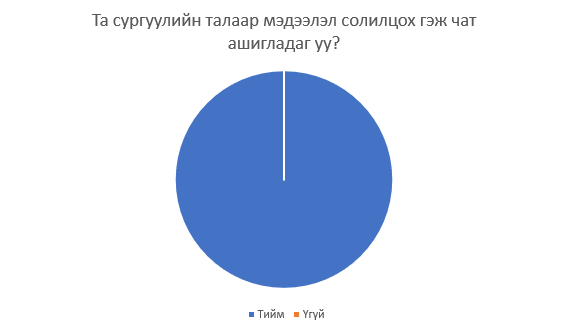
\includegraphics[scale=0.5]{Chart/Chart1}
	\caption[Хэрэглэгчийн судалгаа]{Та сургуулийн талаар мэдээлэл солилцох гэж чат ашигладаг уу?(Асуулга.)}
	\label{fig:Chart1}
\end{figure}

\begin{figure}[htbp]
	\centering
	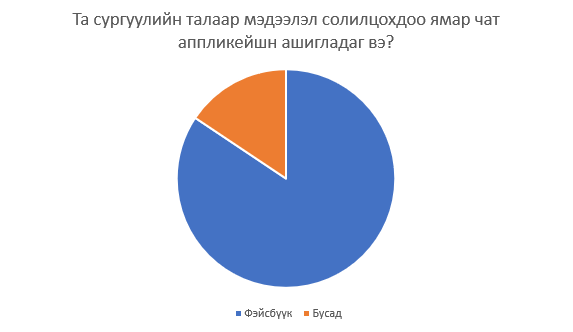
\includegraphics[scale=0.5]{Chart/Chart2}
	\caption[Хэрэглэгчийн судалгаа]{Та сургуулийн талаар мэдээлэл солилцохдоо ямар чат аппликейшн ашигладаг вэ?(Асуулга.)}
	\label{fig:Chart2}
\end{figure}

\begin{figure}[htbp]
	\centering
	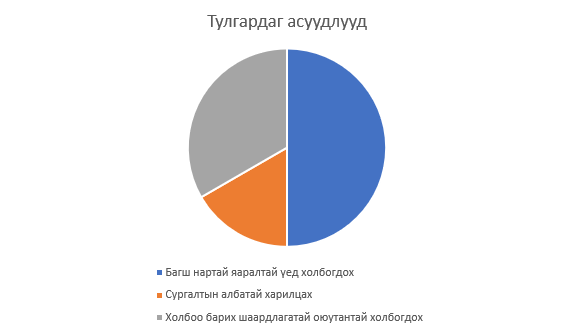
\includegraphics[scale=0.5]{Chart/Chart3}
	\caption[Хэрэглэгчийн судалгаа]{Тулгардаг асуудлууд(Асуулга.)}
	\label{fig:Chart3}
\end{figure}

%-------------------------------------------------------------------------------

\section{Технологийн судалгаа}

\subsection{Ижил төстэй системүүд}
\begin{itemize}
	\item Фэйсбүүк мессенжер (Facebook Messenger) нь 2.27 тэрбум хүн хэргэлдэг. Бүх төрлийн файл дамжуулах боломжтой чат систем.
	\item Вичат (Wechat) ихэвчлэн хятад болон зүүн номхон далайн орны хүмүүс хэргэлдэг. Бүх төрлийн файл дамжуулах боломжтой, мөн төлбөр тооцоо болон нийгмийн бүх хэрэгцээнд ашигладаг
	\item Вайбер (Viber) монголд байгууллагын дотоод холбоонд хүмүүс их ашигладаг.
	\item Ватсап (Whatsapp) америк болон европын орны иргэд их ашигладаг. Хурдан найдвартай нөөц бага ашигладаг систем.
	\item Инстаграм дайрект (Instagram Direct) инстаграм хэрэглэгчид дунд ашигладаг.
	\item Хангаут (Google Hangouts) олон хүн ашигладаггүй ч маш өргөн боломжтой чат болон харилцааны систем.
	\item Скайп (Skype) видео дуудлага, аудио дуудлагын чанар өндөр байгууллагын дотоод харилцаанд их ашигладаг. 
\end{itemize}.
\begin{figure}[htbp]
	\centering
	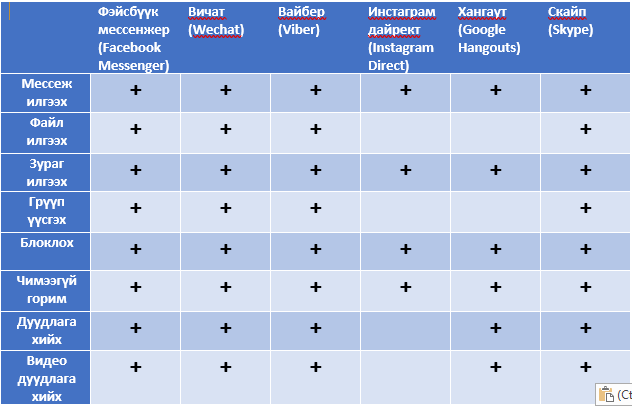
\includegraphics[scale=0.9]{Chart/Chart8}
	\caption[Хэрэглэгчийн судалгаа]{Ижил системүүдийн харьцуулсан хүснэгт}
	\label{fig:Chart3}
\end{figure}

\subsection{MySQL}
MySQL нь холбоост өгөгдлийн санг удирдах систем юм. MySQL хэмээх нэрний хувьд уг системийг санаачлан хөгжүүлэгч Micheal Widenius-ын охины нэр My + SQL(Structed Query Language) гэсэн утгатай ажээ.
Энэ систем нь GNU (General Public License) буюу нээлтэй эхийн систем учир хүссэн хэн бүхэн хөгжүүлэлтэнд оролцож, үнэгүй хэрэглэж болох юм. Эзэмшигч нь алдарт Java-г хөгжүүлсэн Sun MicroSystems компани байсан ба, одоогоор Sun-г Oracle корпораци эзэмших болсон билээ.
Үнэгүй програм хангамжийн өгөгдлийн санг удирдах системд ихэвчлэн MySQL-ийг хэрэглэдэг бөгөөд тэдгээрийн сонгодог жишээ гэвэл Joomla, Drupal, Wordpress, phpBB гэх мэт агуулга удирдах системүүд (CMS-Content Management System), Wikipedia, Facebook, Google гэх мэт томоохон компаниуд хэрэглэдэг юм.
Хөгжүүлэлт нь C/C++ хэл дээр хийгдсэн ба AIX, BSDi, FreeBSD, HP-UX, i5/OS, Linux, Mac OS X, NetBSD, Novell NetWare, OpenBSD, OpenSolaris, eComStation, OS/2 Warp, QNX, IRIX, Solaris, Symbian, SunOS, SCO OpenServer, SCO UnixWare, Sanos, Tru64, Microsoft Windows гэсэн олон үйлдлийн системүүд дээр ажилладаг.
MySQL бол хамгийн өргөн хэрэглээтэй нээлттэй эхийн (Open Source) өгөгдлийн сан удирдах програм юм. Анх 1995 онд зах зээлд гарсан ба с/с++ хэл дээр бичигдсэн. Одоогийн байдлаар 5.7 нь хамгийн сүүлийн хувилбар болон гараад байна. Энэ сүүлийн хувилбар дээр нэмэгдсэн давуу талууд гэвэл 3 дахин хурдан үйл ажиллагаатай болсон мөн натив JSON дэмжигчтэй болсон гэх мэт шинэлэг үйлдлүүд нэмэгдсэн байна.

\subsection{Php}
  Rasmus Lerdorf WWW-д вэб хуудас үүсгэх үедээ өгөгдөл боловсруулах хялбархан арга хайж байгаад 1995 онд PHP хэлийг скрипт хэл байдлаар зохиосон.
PHP нь сервер талын скрипт хэл ба динамик вэб хуудас хийхэд илүү тохиромжтой. Энэ скрипт хэл нь энгийн хэрэглээний вэб сайтаас эхлээд байгууллагын иж бүрэн вэб программ хийж болохоор MySQL мэтийн өгөгдлийн сантай харилцан ажиллах боломжтой.
Хуудас ачаалах үед броузерээр нэг бүрчлэн уншдаг HTML-тэй адилгүй, PHP баримтыг бэлтгэхдээ серверээр урьдчилан боловсруулдаг. PHP код агуулсан хуудас нь хэрэглэгчийн броузерт илгээгдхээс өмнө серверээр боловсруулагдсан байдаг.
PHP хэлний өөр нэг давуу тал бол скриптэн хэл юм. Ихэнх програмчлалын хэлнүүдэд ажиллахын өмнө машины хэл рүү хөрвүүлэх тусгай файлууд /compile/ шаардлагатай байдаг бол PHP хэлний хувьд хөрвүүлэлт хийх шаардлагагүй байдаг тул код засварлах болон шалгахад илүү хурдан байдаг

\subsection{JQuery}
2006 оны эхээр АНУ-ын Нью-Иорк хотын BarCamp-д John Resig хэмээх вэб хөгжүүлэгч залуу jQuery сангийн тухай анх мэдэгджээ. Resig өөрийн вэб сайтдаа: Тухайн үед байгаа сангуудад сэтгэл дундуур байгаагаа, мөн түүнчлэн JavaScript – ий тухай бичилтийг нь багасгаснаар маш их ажил хөнгөвчлөх боломжтой, энгийн үйлдлүүдэд зориулан тусгай хэрэгслүүд нэмэх хэрэгтэй гэж дурдсан байдаг.
Хөгжүүлэх нийгэмлэгт jQuery нь томоохон амжилт авчирсан төдийгүй улмаар маш хурдтай хөгжсөн. Бусад хөгжүүлэгчид сан боловсронгуй болгоход тусалж эхэлснээр jQuery – гийн анхны хувилбар 1.0 нь 2006 оны 8-р сарын 26- нд гарсан.
Түүнээс хойш jQuery 3.1.1 хувилбар гарсан ба хөгжүүлэлтийн нийгэмлэгээс plug-in –ийг маш ихээр оруулсан. Plug-in нь jQuery – ийн сангийн цөм хэсэг биш харин нэмэлт хэрэгсэл юм. 
jQuery – гийн давуу талууд нь:
\begin{itemize}
\item Файлын хэмжээ бага
\item Маш энгийн бичилттэй
\item Холбоо бүхий method – уудтай
\item Санг өргөтгөх plug-in нь энгийн бүтэцтэй
\item Асар том онлайн нийгэмлэгтэй
\item JQueryUI мэтийн jQuery – гийн нэмэлт сонголтуудтай
\end{itemize}

%-------------------------------------------------------------------------------